\section{Diseño del sistema}

\subsection{Conceptos}

\begin{itemize}
    \item Necesidad: Es el resultado de una transformación de uno a más conceptos en un expectativa para el cumplimiento de una función con cierto o dentro de cierto rendimiento. Indicadores de calidad (KPI).
    
    \item Requerimiento: Es el resultado de una transformación de una o más necesidades en una obligación para cumplir cierta función dentro de las cotas establecidas.
\end{itemize}

 \subsection{Clasificación general de requerimientos}
 \begin{enumerate}
     \item Requerimientos funcionales: Algo que el sistema debe hacer o proveer.
     
     \item Requerimientos no funcionales: Alguna propiedad o atributo que el sistema debe tener pero que no se modifica el comportamiento o cumplimiento de las funciones que desempeña (deben cumplirse, pero no afecta la funcionalidad).
     
     \item Restricción: Son las fronteras en las que el sistema debe operar. Comúnmente se enlistan dentro de los requerimientos funcionales y no-funcionales. 
 \end{enumerate}
 
 Un requerimiento debe definir qué es lo que debe hacer, no como hacerlo.
 
 ¿Por qué se necesitan?
 \begin{itemize}
     \item Para definir el alcance del proyecto.
     
     \item Para asegurar el cumplimiento de las expectativas.
     
     \item Para poder reportar un progreso.
     
     \item Para medir el avance en el proceso del diseño.
 \end{itemize}
 
 Principales características
 \begin{enumerate}
     \item Necesario
     \item Singular
     \item Correcto
     \item inequívoco
     \item Realizable
     \item Completo: Tenga un rango
     \item Ajustable: Que se pueda medir
 \end{enumerate}
 
 \subsection{Términos}
 \begin{itemize}
     \item Necesidad: Expectativa no tangible
     \item Requerimiento: Algo acotado
     \item Especificación: Valor final medible
     \item Diseñar: Cumplir requerimientos
     \item Necesidad no funcional: Son aquellas que no afectan la función principal
 \end{itemize}
 
\begin{figure}[h!]
    \centering
        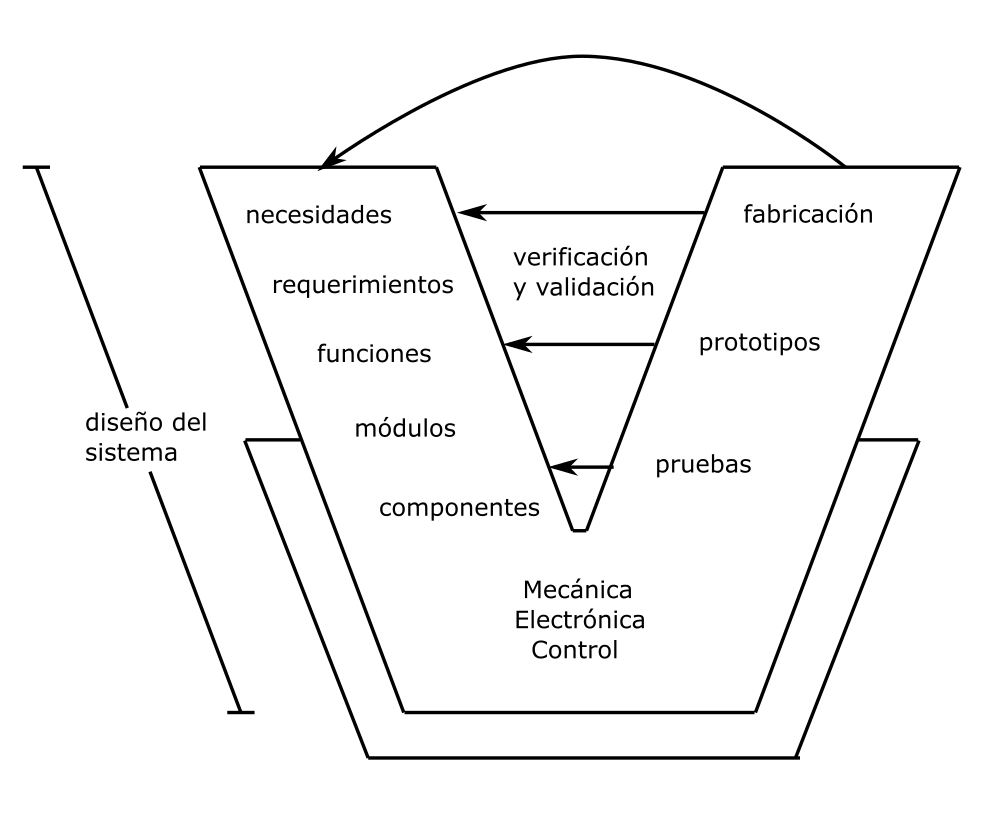
\includegraphics[scale=0.5]{Proyecto Integrador Figuras/10 VDI-2206.png}
        \caption{VDI-2206}
\end{figure}